% !Tex root=main.tex

\section{Background}
\label{sec:background}

In this section, we provide the background on learning-based invariant synthesis.
In particular, we briefly recapitulate the Horn-ICE learning framework (in Section~\ref{sec:horn-ICE}) and discuss the \houdini algorithm (in Section~\ref{sec:houdini}).

To make the Horn-ICE framework mathematically precise, let $P$ be the program (with assertions) under consideration and $\mathcal C$ the set of all program configurations of $P$.
Furthermore, let us fix a finite set $\mathcal P$ of \emph{predicates}
$p \colon \mathcal C \to \mathbb B$ over the program configurations, where $\mathbb B = \{ 0, 1 \}$ is the set of Boolean values (with $1$ interpreted as \textit{true} and $0$ as \textit{false}).
These predicates capture interesting properties of the program and serve as the basic building blocks for constructing invariants.
We assume that the values of these predicates can either be obtained directly from the program configurations or that the program is instrumented with ghost variables that track the values of the predicates at important places in the program (e.g., at the loop header and immediately after the loop).
As notational convention, we write $c \models p$ if $p(c) = 1$ and $c \not\models p$ if $p(c) = 0$.
Moreover, we lift this notation to formulas $\varphi$ over $\mathcal P$ (i.e., arbitrary Boolean combinations of predicates from $\mathcal P$) and use $c \models \varphi$ ($c \not\models \varphi$) to denote that $c$ satisfies $\varphi$ ($c$ does not satisfy $\varphi$), that is defined as usual. 
%We assume that one can evaluate predicates on a program configuration in constant time.

To simplify the presentation in the remainder of this paper, we use conjunctions $p_1 \land \cdots \land p_n$ of predicates over $\mathcal P$ and the corresponding sets $\{ p_1, \ldots, p_n \} \subseteq \mathcal P$ interchangeably.
In particular, for a (sub-)set $X = \{ p_1, \ldots, p_n \} \subseteq \mathcal P$ of predicates and a program configuration $c \in \mathcal C$, we write $c \models X$ if and only if $c \models p_1 \land \cdots \land p_n$.


%---------- The Horn-ICE Learning Framework ----------
\subsection{The Horn-ICE Learning Framework}
\label{sec:horn-ICE}

The Horn-ICE learning framework~\cite{DBLP:conf/tacas/ChampionC0S18,DBLP:journals/pacmpl/EzudheenND0M18} is a general framework for learning inductive invariants in a black-box setting.
We here assume without loss of generality that the task is to synthesize a single invariant.
In the case of learning multiple invariants, say at different program locations, one can easily expand the given predicates to predicates of the form $(\mathit{pc} = l) \rightarrow p$ where $\mathit{pc}$ refers to the program counter, $l$ is the location of an invariant in the program, and $p \in \mathcal P$.
Learning a conjunctive invariant over this extended set of predicates then corresponds to learning multiple conjunctive invariants at the various locations. % in the program.

As sketched in Figure~\ref{fig:horn-ice-learning}, this framework consists of two distinct entities---the \emph{learner} and the \emph{teacher}---and proceeds in rounds.
%In each round, the learner proposes a candidate invariant $\varphi$ for the program, and the teacher, with access to a verification engine, checks whether the proposed invariant proves the program correct. 
%If this is the case, the learning process stops, and this invariant is returned.
%If, on the other hand, the invariant is not adequate to prove the program correct, the teacher replies with concrete program configurations (so called \emph{counterexamples}), which the learner then uses in the next round to refine its conjecture.
%Note that the key feature of this framework is that the learner is completely agnostic of the program and the specification---it is simply constrained to learn some predicate that is consistent with the counterexamples given by the teacher.
%
In each round, the teacher receives a candidate invariant $\varphi$ from the learner and checks whether $\varphi$ proves the program correct.
Should $\varphi$ not be adequate to prove the program correct, the learner replies with a counterexample, which serves as a means to correct inadequate invariants and guide the learner towards a correct one.
More precisely, a counterexample takes one of three forms:\footnote{By abuse of notation, we write $c \models \alpha$ ($c \not\models \alpha$) to denote that $c$ satisfies (violates) the formula $\alpha$ even if $\alpha$ contains predicates that do not belong to $\mathcal P$.}
\begin{itemize}
    \item If the pre-condition $\alpha$ of the program does not imply $\varphi$, then the teacher returns a \emph{positive counterexample} $c \in \mathcal C$ such that $c \models \alpha$ but $c \not \models \varphi$.
    %
    \item If $\varphi$ does not imply the post-condition $\beta$ of the program, then the teacher returns a \emph{negative counterexample} $c \in \mathcal C$ such that $c \models \varphi$ but $c \not \models \beta$.
    %
     \item If $\varphi$ is not inductive, then the teacher returns a \emph{Horn counterexample} $(\{ c_1, \ldots, c_n \}, c) \in 2^\mathcal C \times \mathcal C$ such that $c_i \models \varphi$ for each $i \in \{ 1, \ldots, n \}$ but $c \not\models \varphi$. (We encourage the reader to think of Horn counterexamples as constraints of the form $(c_1 \land \cdots \land c_n) \rightarrow c$.)
\end{itemize}

\begin{figure}[t]
    \centering
    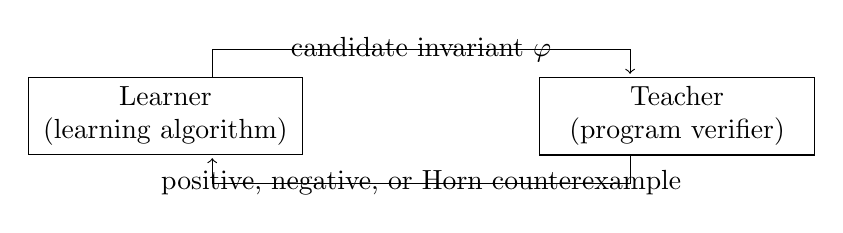
\begin{tikzpicture}
        \node[draw, text width=32.5mm, align=center, anchor=east] (learner) at (0, 0) {Learner \\ (learning algorithm)};
        \node[draw, text width=32.5mm, align=center, anchor=west] (teacher) at (3, 0) {Teacher \\ (program verifier)};
        
        \begin{scope}[->, shorten >= 1pt]
            \draw (learner.40) -- ++(0, .35) -| node[near start] {candidate invariant $\varphi$} (teacher.140);
            \draw (teacher.220) -- ++(0, -.35) -| node[near start] {positive, negative, or Horn counterexample} (learner.320);
        \end{scope}
    \end{tikzpicture}
    \caption{The Horn-ICE learning framework~\cite{DBLP:conf/tacas/ChampionC0S18,DBLP:journals/pacmpl/EzudheenND0M18}}
    \label{fig:horn-ice-learning}
\end{figure}

A teacher who returns counterexamples as described above always enables the learner to make \emph{progress} in the sense that every counterexample it returns is inconsistent with the current conjecture.
Moreover, the Horn-ICE framework requires the teacher to be \emph{honest}, meaning that each counterexample needs to be consistent with \emph{all} inductive invariants that prove the program correct (i.e., the teacher does not rule out possible solutions).
Finally, note that such a teacher can indeed be built since program verification can be stated using \emph{constrained Horn clauses}~\cite{DBLP:conf/pldi/GrebenshchikovLPR12}.
When the candidate invariant does not make such clauses true, some Horn clause must fail, and the teacher can find a Horn counterexample using a logic solver (positive counterexamples arise when the left-hand-side of the Horn counterexample is empty, while negative counterexamples arise when the left-hand-side has one element and the-right-hand side is \emph{false}).


The objective of the learner, on the other hand, is to construct a formula $\varphi$ over $\mathcal P$ from the counterexamples received thus far.
For the sake of simplicity, we assume that the learner collects all counterexamples in a data structure $\mathcal S = (S_+, S_-, S_H)$, called \emph{Horn-ICE sample}, where
\begin{enumerate*}[label={(\alph*)}]
    \item $S_+ \subseteq \mathcal C$ is a finite set of positive counterexamples,
    \item $S_- \subseteq \mathcal C$ is a finite set of negative counterexamples, and
    \item $S_H \subseteq 2^\mathcal C \times \mathcal C$ is a finite set of Horn counterexamples.
\end{enumerate*}
To measure the complexity of a sample, we define its \emph{size}, denoted by $|\mathcal S|$, to be $|S_+| + |S_-| + \sum_{(L, c) \in S_H} (|L| + 1)$.

Given a Horn-ICE sample $\mathcal S = (S_+, S_-, S_H)$, the learner's task is then to construct a formula $\varphi$ over $\mathcal P$ that is \emph{consistent} with $\mathcal S$ in that
\begin{enumerate*}[label={(\alph*)}]
    \item $c \models \varphi$ for each $c \in S_+$,
    \item $c\not \models \varphi$ for each $c \in S_-$, and
    \item for each $(\{ c_1, \ldots, c_n \}, c) \in S_H$, if $c_i \models \varphi$ for all $i \in \{ 1, \ldots, n \}$, then $c \models \varphi$.
\end{enumerate*}
This task is called \emph{passive Horn-ICE learning}, while the overall learning setup can be though of as \emph{iterative (or online) Horn-ICE learning}.
In the special case that the learner produces conjunctive formulas, we say that a set $X \subseteq \mathcal P$ is consistent with $\mathcal S$ if and only if the corresponding conjunction $\bigwedge_{p \in X} p$ is consistent with $\mathcal S$


In general, the Horn-ICE learning framework permits arbitrary formulas over the predicates as candidate invariants.
In this paper, however, we exclusively focus on conjunctive formulas (i.e., conjunctions of predicates from $\mathcal P$). % \textcolor{orange}{and assume that the set of predicates is finite}.
In fact, conjunctive invariants form an important subclass in practice as they are sufficient to prove many programs correct~\cite{DBLP:conf/fm/FlanaganL01,DBLP:conf/tacas/Neider0MS018} (also see our experimental evaluation in Section~\ref{sec:experiments}).
Moreover, once can design efficient learning algorithms for conjunctive Boolean formulas, as we show next.


%---------- Houdini ----------
\subsection{\houdini as a Horn-ICE Learning Algorithm}
\label{sec:houdini}

\houdini~\cite{DBLP:conf/fm/FlanaganL01} is typically seen as a particular way to synthesize invariants, but is best understood as a passive Horn-ICE learner for conjuncts, as we describe below.
In fact, \houdini is similar to the classical PAC learning algorithm for conjunctions~\cite{Kearns:1994:ICL:200548}, but extended to work with Horn counterexamples as well.
%In every round, the \houdini algorithm learns the \emph{largest} set of conjuncts that satisfies the current positive and implication samples (thus, it can never misclassify a negative sample if a consistent conjunction exists), and hence learns, in the iterative setting, the invariant that can be expressed using the largest set of conjuncts.

We now describe the \houdini algorithm, as it will be used in the design of the \sorcar algorithm that we develop.
Given a Horn-ICE sample $\mathcal S = (S_+, S_-, S_H)$, \houdini computes the largest conjunctive formula $X \subseteq \mathcal P$ in terms of the number of predicates in $X$ (i.e., the semantically smallest set of program configurations expressible by a conjunctive formula) that is consistent with $\mathcal S$.
Starting with the set $X = \mathcal P$ of all predicates, the \houdini algorithm proceeds as follows:
\begin{enumerate}
    \item \label{item:houdini-1} \houdini removes all predicates $p \in X$ from $X$ that violate a positive counterexample (i.e., there exists a positive counterexample $c \in S_+$ such that $c \not\models p$).
    The result is the unique largest set $X$ of predicates---alternatively the largest conjunctive formula---that is consistent with $S_+$ (i.e., $c \models X$ for all $c \in S_+$).
    %
    \item \label{item:houdini-2} \houdini checks whether all Horn counterexamples are satisfied.
    If a Horn counterexample $(\{ c_1, \ldots, c_n \}, c) \in S_H$ is not satisfied, it means that each program configuration $c_i$ of the left-hand-side satisfies $X$, but the configuration $c$ on the right-hand-side does not.
    However, $X$ corresponds to the semantically smallest set of program configurations expressible by a conjunctive formula that is consistent with $S_+$.
    Moreover, all program configurations $c_i$ on the left-hand-side of the Horn counterexample also satisfy $X$.
    Thus, the right-hand-side $c$ necessarily has to satisfy $X$ as well (otherwise $X$ would not satisfy the Horn counterexample).
    To account for this, \houdini adds $c$ as a new positive counterexample to $S_+$.
    %
    \item \label{item:houdini-3} \houdini repeats Steps~\ref{item:houdini-1} and \ref{item:houdini-2} until a fixed point is reached. Once this happens, $X$ is the unique largest set of predicates that is consistent with $S_+$ and $S_H$.
\end{enumerate}
Finally, \houdini checks whether each negative counterexample violates $X$ (i.e., $c \not\models X$ for each $c \in S_-$).
If this is the case, $X$ is the largest set of predicates that is consistent with $\mathcal S$; otherwise, no consistent conjunctive formula exists.

%Given a Horn-ICE sample $\mathcal S = (S_+, S_-, S_H)$, \houdini computes the largest conjunctive formula $\varphi$ in terms of the number of predicates occurring in $\varphi$ (i.e., the semantically strongest conjunctive formula) that is consistent with $\mathcal S$ in the following way.
%First, it computes the largest conjunction $\varphi$ that is consistent with the positive examples (i.e., $c \models \varphi$ for all $c \in S_+$); note that this conjunction is unique.
%Next, \houdini checks whether the implications are satisfied.
%If this is not the case, then we know for each non-satisfied implication $(\vec{v}_1, \vec{v}_2) \in S_\Rightarrow$ that $\vec{v}_2$ has to be classified positively because $\vec{v}_1$ belongs to every set that includes $S_+$.
%Hence, \houdini adds all such $\vec{v}_2$ to $S_+$, resulting in a new set $S'_+$.
%Subsequently, it constructs the largest conjunction $\varphi'$ that is consistent with the positive examples in $S'_+$ (i.e., $\vec{v} \models \varphi'$ for all $\vec{v} \in S'_+$).
%\houdini repeats this procedure until it arrives at the largest conjunctive formula $\varphi^\ast$ that is consistent with $S_+$ and $S_\Rightarrow$ (again, note that this set is unique).
%Finally, \houdini checks whether each negative example violates $\varphi^\ast$  (i.e., $\vec{v} \not\models \varphi^\ast$ for all $\vec{v} \in S_-$).
%If this is the case, $\varphi^\ast$ is the largest conjunctive formula over $\mathcal B$ that is consistent with $\mathcal S$; otherwise, no consistent conjunctive formula exists.

It is not hard to verify that the time \houdini spends in each round is \emph{polynomial} in the number of predicates and the size of the Horn-ICE sample (provided predicates can be evaluated in constant time).
Furthermore, \houdini is guaranteed to converge in at most $|\mathcal P|$ rounds when used in an iterative setting, or it reports that no conjunctive invariant over $\mathcal P$ exists.

The property that \houdini converges in at most $|\mathcal P|$ rounds is of great importance in practice.
We can, for instance, in every round learn the \emph{smallest} set of conjuncts satisfying the sample, say using a SAT solver.
Doing so would not significantly increase the time taken for learning in each round (thanks to highly-optimized SAT solvers), but the worst-case number of iterations to converge to an invariant becomes exponential.
An exponential number of rounds, however, makes learning invariants often intractable in practice (we implemented such a SAT-based learner, but it performed poorly on our set of benchmarks).
Hence, it is important to keep the number of iterations small when learning invariants.
%, and as we shall show in experiments later, is very advantageous in practice when learning from a large set of predicates.  
Note that the \houdini algorithm does not use \emph{negative examples} to learn formulas, and hence is \emph{not property-driven} (negative examples come from configurations that lead to violating assertions).
The \sorcar algorithm, which we describe in the next section 
%uses negative examples, is property driven, and still has the guarantee of linear number of rounds.
has this feature, but at the same time has a bias to producing small conjunctive invariants.
